\chapter{Document Preprocessing}
In previous chapters we have analyzed how to construct query, how to compress result,
now we will explain how to process document that has to be indexed.

Given documents to parse them we have to discover format, language and character set
used and each of them is a classification problem, but usually we use some heuristics.

After we have parsed document we tokenize them and we have the following definitions:
\begin{defi}
     Token is an istance of a sequence of characters
\end{defi}
Each such token is now a candidate for an index entry, after further processing,
that we will now present.

Sometimes there are some issues like "San Francisco" should be $1$ or $2$ tokens, or
also how to deal with hypens, apostrophe and usually this is done based with word
and is language dependent.

Another preprocessing step is to remove \emph{Stop words}, most common words in
document, and the intuition behind is that they have little semantic content
(the, a, and, to, be) and there are a lot of them ($\sim 30\%$ of postings 
for top $30$ words).\newline
Nowadays good compression techniques has reduced the space necessary to include also
stopwords and with good query optimations it is required only a small more time also
to consider it, so usually the stop words are not deleted.

We need also to “normalize” terms in indexed text and query words into the same form
so we want to match U.S.A. and USA, so we most commonly implicitly define 
\emph{equivalence classes} of terms; another preprocessing is to reduce all letters
to lower case (there is an exception to consider upper case in midsentence but often
best to lowercase everythin, since users will use lowercase regardless
of ‘correct’ capitalization).

\emph{Thesauri} is how to handle synonyms and homonyms and there are two ways to consider it: by hand-constructed equivalence classes we can rewrite to form 
equivalence-class terms and when the document contains automobile, index it 
under car-automobile (and vice-versa) or we can expand a query, so when the query
contains automobile, look under car as well.

\emph{Stemming} is the process to reduce terms to their “roots” before indexing and
suggest crude affix chopping (it is language dependent and for example 
automate(s), automatic, automation all reduced to automat).

\emph{Lemmatization} reduce inflectional/variant forms to base form (so for example
am, are,is became be)and Lemmatization implies doing “proper” reduction to 
dictionary headword form.

Many of the above features embody transformations that are language-specific and
often, application-specific and these are “plug-in” addenda to indexing.

\section{Statistical Properties of Text}
Tokens are not distributed uniformly, they follow the so called \emph{Zipf Law},
so few tokens are very frequent, a middle sized set has medium frequency and 
many are rare; the first $100$ tokens sum up to $50\%$ of the text,
and many of them are stopwords.

$k$-th most frequent token has frequency $f(k)$ approximately $1/k$, equivalently,
the product of the frequency $f(k)$ of a token and its rank $k$ is a constant
\[ k * f(k) = c \]
The number of distinct tokens grows, following with the so called \emph{Heaps Law}
\[ T = kn^b\]
where $b$ is typically $0.5$ and $n$ is the total number of tokens.\newline
The average token length grows as $\Theta(\log n)$ and interesting words 
are the ones with medium frequency (Luhn).

\section{Keyword extraction}
To extract keyword that should be consider as a single token we have several approaches that we can consider:
\begin{enumerate}
    \item Use frequency and POS (Part of Speech) tagging to obtain keywords, 
	  as can be viewed in figure \ref{img:posFrequency}.

	  \begin{figure}
		  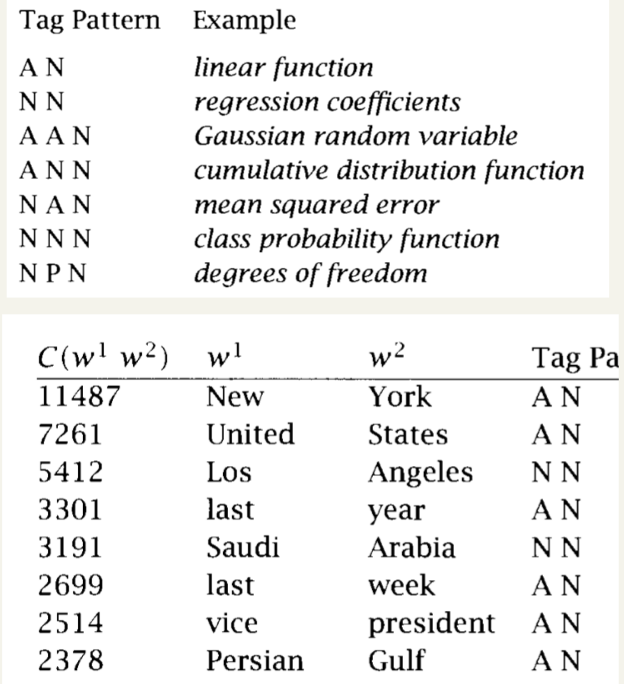
\includegraphics[width=\textwidth]{Images/posFrequency}
		  \caption{Frequency and POS tagging approach}
		  \label{img:posFrequency}
	  \end{figure}

    \item Often the words are not adjacent to each other and to find keyword we 
	  compute the mean and the variance of the distance, 
	  by restricting within a window, as it is possible to note in figure
	  \ref{img:meanDistance} and \ref{img:exampleDistance}.
	  If $s$ is large, the collocation is not interesting, instead if
	  $d > 0$ and $s$ very small we have interesting new keyword.

	  \begin{figure}
		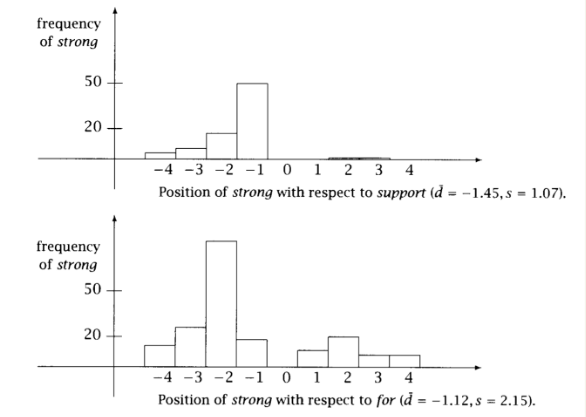
\includegraphics[width=0.7\textwidth]{Images/meanDistance}
		\caption{Mean and Variance between Strong and some words}
		\label{img:meanDistance}
	  \end{figure}

	  \begin{figure}
		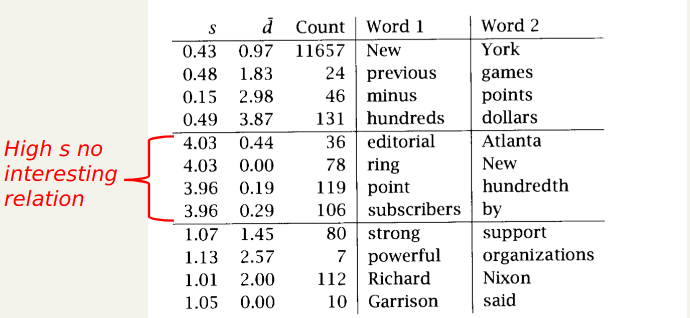
\includegraphics[width=0.7\textwidth]{Images/exampleMeanDistance}
		\caption{Example of Mean and Variance distance}
		\label{img:exampleDistance}
	  \end{figure}
    \item Pearson Chi-Square test statistics that follow a chi-squared distribution
	  arise from an assumption of independent normally distributed data,
	  which is valid in many cases due to the central limit theorem and 
	  we use $p$-value to reject the null hypothesis.

    \item \emph{RAKE} (Rapid Automatic Keyword Extraction) works on single 
	  (not much long) documents and is easily applicable to new domains, fast
	  and unsupervised.\newline
	  The Key observation of this approach is that keywords frequently contain
	  multiple words but rarely contain punctuation or stop words.

	  The input parameters are the following:
	  \begin{itemize}
		\item a set of word delimiters
		\item a set of phrase delimiters
		\item a list of stop words (or stoplist).
	   \end{itemize}
	   The RAKE approach has the following 4 step:
	   \begin{description}
		\item [Step $\#1$: ] document is split into an array of words by the specified word delimiters and 
		      this array is split into sequences of contiguous words at phrase delimiters and then stop word.

		      Words within a sequence are considered a candidate keyword, as we can see in figure 
		      \ref{img:rake}.

		      \begin{figure}
			      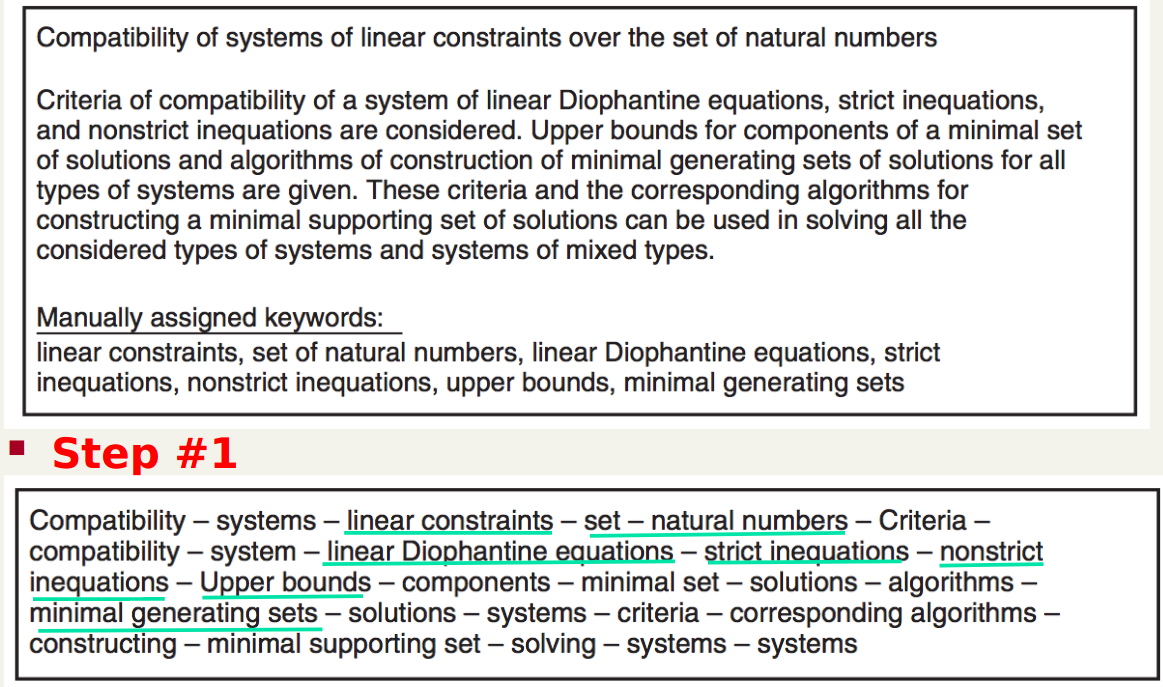
\includegraphics[width=\textwidth]{Images/rake}
			      \caption{Extraction of Candidate keywords using RAKE}
			      \label{img:rake}
		      \end{figure}

		\item [Step \#2: ] compute the table of co-occurrences and we use few metrics:
			          $freq(w)$ = total frequency on diagonal and $deg(w)$ sum over row.\newline
                                  Final score is the sum of $deg(w)/freq(w)$ for the constituting words $w$ 
				  of a keyword and in figure \ref{img:scoringCandidate} is possible to know how
				  to compute the scoring Candidate keywords.

			\begin{figure}
				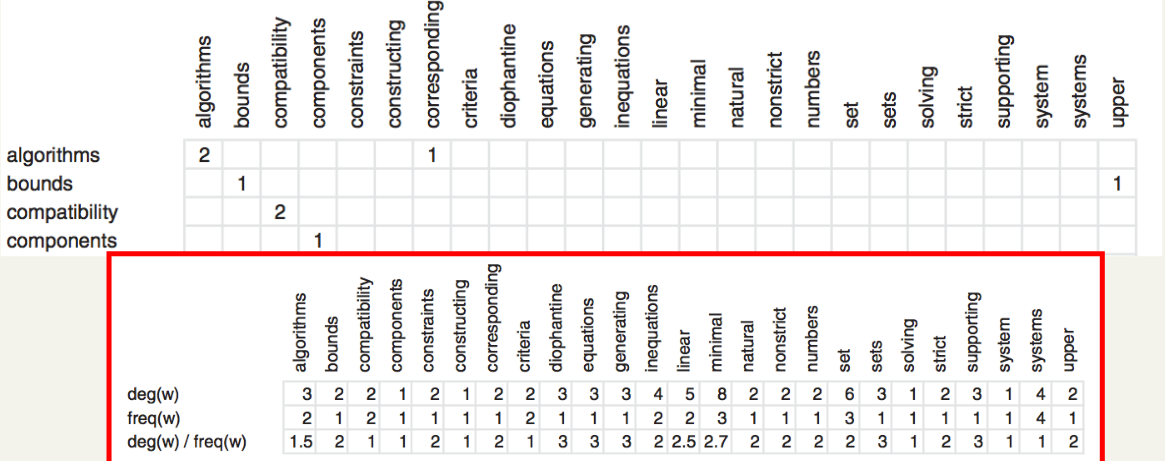
\includegraphics[width=\textwidth]{Images/rakeScoring}
				\caption{Calculation of Scoring of Candidate keywords}
				\label{img:scoringCandidate}
			\end{figure}
		\item [Step \#3: ] identifies keywords that contain interior stop words such as axis of evil and 
			looks for pairs of keywords that adjoin one another at least twice in the same document
			and in the same order.\newline
			The score for the new keyword is the sum of its member keyword scores, as can be viewed
			in figure \ref{img:listScoring}.

			\begin{figure}
				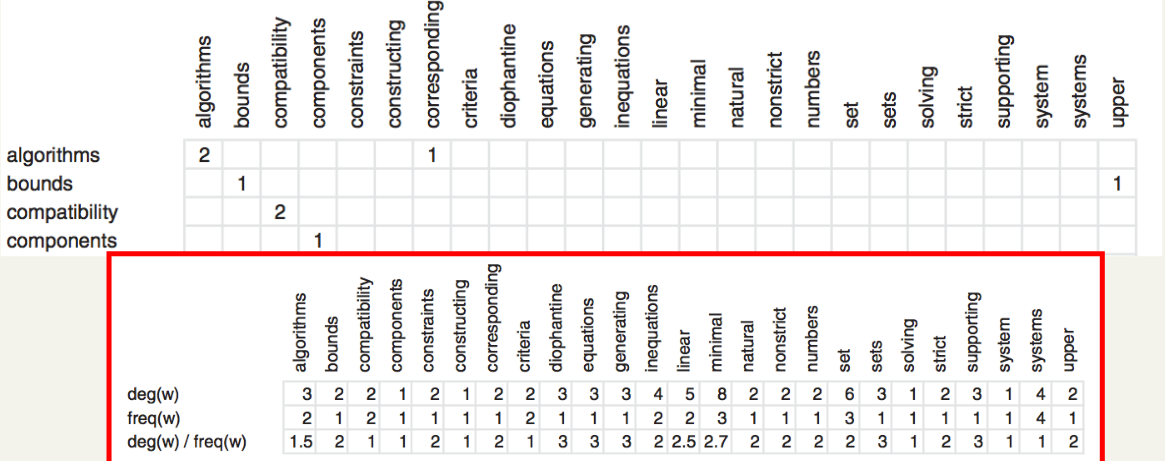
\includegraphics[width=\textwidth]{Images/rakeScoring}
				\caption{Sorted Scoring of RAKE approach}
				\label{img:listScoring}
			\end{figure}
		\item [Step \#4: ] we select the top one-third of sorted list of scoring obtained in previous steps
			and in figure \ref{img:rakeScoring} is possible to compare results obtained by RAKE and 
			by manual keyword extraction.

			\begin{figure}
				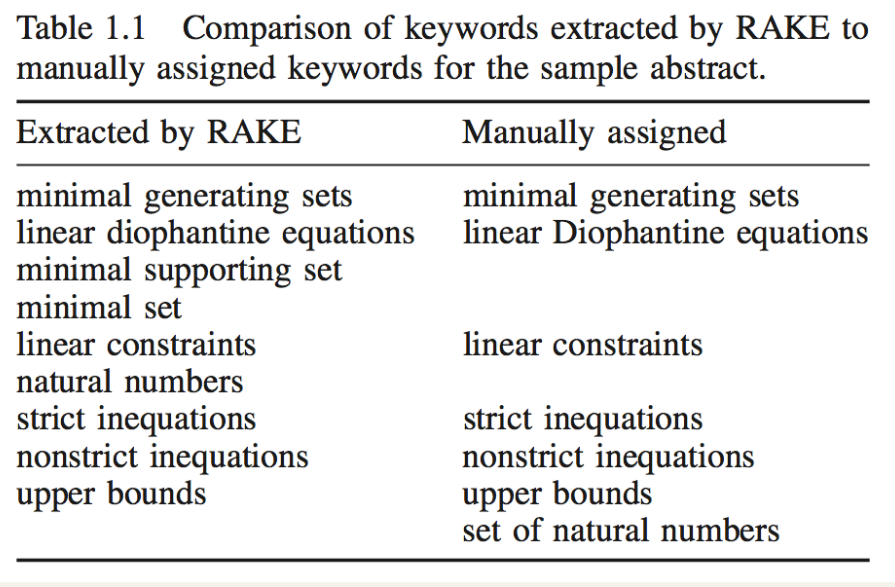
\includegraphics[width=\textwidth]{Images/rakeComparison}
				\caption{Results obtained by Rake and manual extraction}
				\label{img:rakeScoring}
			\end{figure}

	   \end{description}
\end{enumerate}

